\documentclass{article}
\usepackage{amsmath,amsthm,amssymb}
\usepackage {mathtext}
\usepackage{amsfonts} 
\usepackage[T1,T2A]{fontenc}
\usepackage[utf8]{inputenc}
\usepackage [english, russian] {babel}
\usepackage[babel=true]{microtype}
\usepackage{caption}
\usepackage{subcaption}
\captionsetup[table]{position=t,justification=raggedleft,slc=off}
\setlength{\abovecaptionskip}{0pt}
\usepackage {geometry}
\usepackage{graphicx}
\usepackage{multirow}
\usepackage{booktabs}
\usepackage{pgfplots}
\pgfplotsset{compat=1.18}
\geometry{top=2cm, bottom=2cm, left=2cm, right=1cm}
\title{Отчёт о лабораторной работе №2.2.6. \\ Определение энергии активации по температурной зависимости вязкости жидкости}
\author{Павел Рудачихин, группа Б04-507}
\date{01.04.2026}
\begin{document}
\maketitle
	\section*{Аннотация}
		
		
		\hspace{4mm} В данной работе измеряется энергия активации молекул глицерина по зависимости его вязкости от температуры, которая снимается по скорости падения шариков.
		
		
		\textbf{Цель работы:}  1) измерение скорости падения шариков при разной температуре жидкости; 2) вычисление вязкости жидкости по закону Стокса и расчет энергии активации.
		
		
		\textbf{Оборудование:}  стеклянный цилиндр с исследуемой жидкостью (глицерин); термостат; секундомер; микроскоп; шарики диаметром около 1 мм.
		
		
		\textbf{Методы:} измерение диаметра с помощью микроскопа, измерение времени секундомером, построение графика линейной зависимости и определение углового коэффициента по методу наименьших квадратов.

	
	 
	
\section*{Теоретические сведения}
	
	\hspace{4mm} В жидкости присутствует ближний, но не дальний порядок:	расположение молекул упорядочено в небольших объемах, но порядок перестает замечаться при увеличении расстояния. Для того чтобы перейти в новое состояние, молекула должна преодолеть участки с большой потенциальной энергией, превышающей среднюю тепловую энергию молекул. Для этого тепловая энергия молекул должна увеличиться на некоторую величину $W$, называемую \textit{энергией активации}. Вследствие этого переходы молекул из одного положения равновесия в другое происходят сравнительно редко и тем реже, чем больше энергия активации.
	
	
	Отмеченный характер движения молекул объясняет большую (по сравнению с газами) вязкость жидкостей. В газах вязкость объясняется происходящим при тепловом движении молекул переносом количества направленного движения. В жидкостях такие переходы существенно замедлены. Количество молекул, имеющих энергии больше $W$, в соответствии с формулой Больцмана экспоненциально зависит от $W$. Температурная зависимость вязкости жидкости выражается формулой
	
	\begin{equation}
		\eta = A e^{W / kT}
	\end{equation}
	
	Из формулы (1) следует, что вязкость жидкости при повышении температуры должна резко уменьшаться. Если отложить на графике логарифм вязкости $\ln \eta$ в зависимости от $1/T$, то должна получиться прямая, по угловому коэффициенту которой можно определить энергию активации молекулы W исследуемой жидкости. Экспериментальные исследования показывают, что в небольших температурных интервалах эта формула неплохо описывает изменение вязкости с температурой.
	
	
	Для исследования температурной зависимости вязкости жидкости в данной работе используется метод Стокса, основанный на измерении скорости свободного падения шарика в жидкости. Стоксом было получено строгое решение задачи о ламинарном обтекании шарика безграничной жидкостью. В этом случае сила сопротивления $F$ определяется формулой
	
	\begin{equation}
		F_s = 6 \pi \eta r v
	\end{equation}
	
	
	На падающий в вязкой жидкости шарик действуют три силы: сила тяжести, сила Архимеда и сила вязкости.
	
	\begin{equation*}
		F_A = \rho_l g V, F_g = mg = \rho g V
	\end{equation*}
	
	По второму закону Ньютона
	
	\begin{equation*}
		m\dot{v} = - F_A + F_g - F_s, 
	\end{equation*}
	
	\begin{equation}
		\rho V \dot{v} = (\rho_l - \rho) g V - 6 \pi \eta r v
	\end{equation}
	
	где $V$ - объем шарика, $\rho$ - его плотность, $\rho_l$ - плотность жидкости. Решая это уравнение, находим
	
	\begin{equation}
		v(t) = u - (u - v_0) \exp(-\frac{t}{\tau})
	\end{equation}
	
	где $v_0 = v(0)$ - скорость в начальный момент времени, $u$ - установившаяся скорость, определяемая так:
	
	\begin{equation*}
		u = \frac{Vg (\rho - \rho_l)}{6 \pi \eta r} = \frac{2}{9} g r^2 \frac{\rho - \rho_l}{\eta}
	\end{equation*}
	
	$\tau$ - время достижения установившейся скорости, т.е. время релаксации:
	
	\begin{equation*}
		\tau = \frac{V \rho}{6 \pi \eta r} = \frac{2}{9} \frac{\rho r^2}{\eta}
	\end{equation*}
	
	Таким образом можно найти вязкость жидкости:
	
	\begin{equation}
		\boxed{\eta = \frac{2}{9} g r^2 \frac{\rho - \rho_l}{u}}
	\end{equation}
	
	Результаты опыта имеет смысл обрабатывать лишь в том случае, если значения $\eta$ не обнаруживают систематической зависимости от $r$. Если такая зависимость наблюдается, то чаще всего это связано с влиянием стенок сосуда. В этом случае вместо формулы (5) следует использовать более точную формулу:
	
	\begin{equation}
	\eta = \frac{2}{9} g r^2 \frac{\rho - \rho_l}{(1 +2,4\frac{r}{R})u}
	\end{equation}	
	
	где $R$ - радиус сосуда.
	
	
	Характер обтекания определяется числом Рейнольдса
	
	\begin{equation*}
		\mathtt{Re} := \frac{v r \rho_l}{\eta}
	\end{equation*}
	
	Течение считается ламинарным при числе Рейнольдса меньше 10.
	
	Интегрируя (4), можно найти путь, полагая $v_0 \approx 0$:
	
	\begin{equation}
		S = u\tau (\frac{t}{\tau} - 1 + \exp(-\frac{t}{\tau}))
	\end{equation}
	
\section*{Экспериментальная установка}
	
	\begin{figure}[h!]
		\centering
		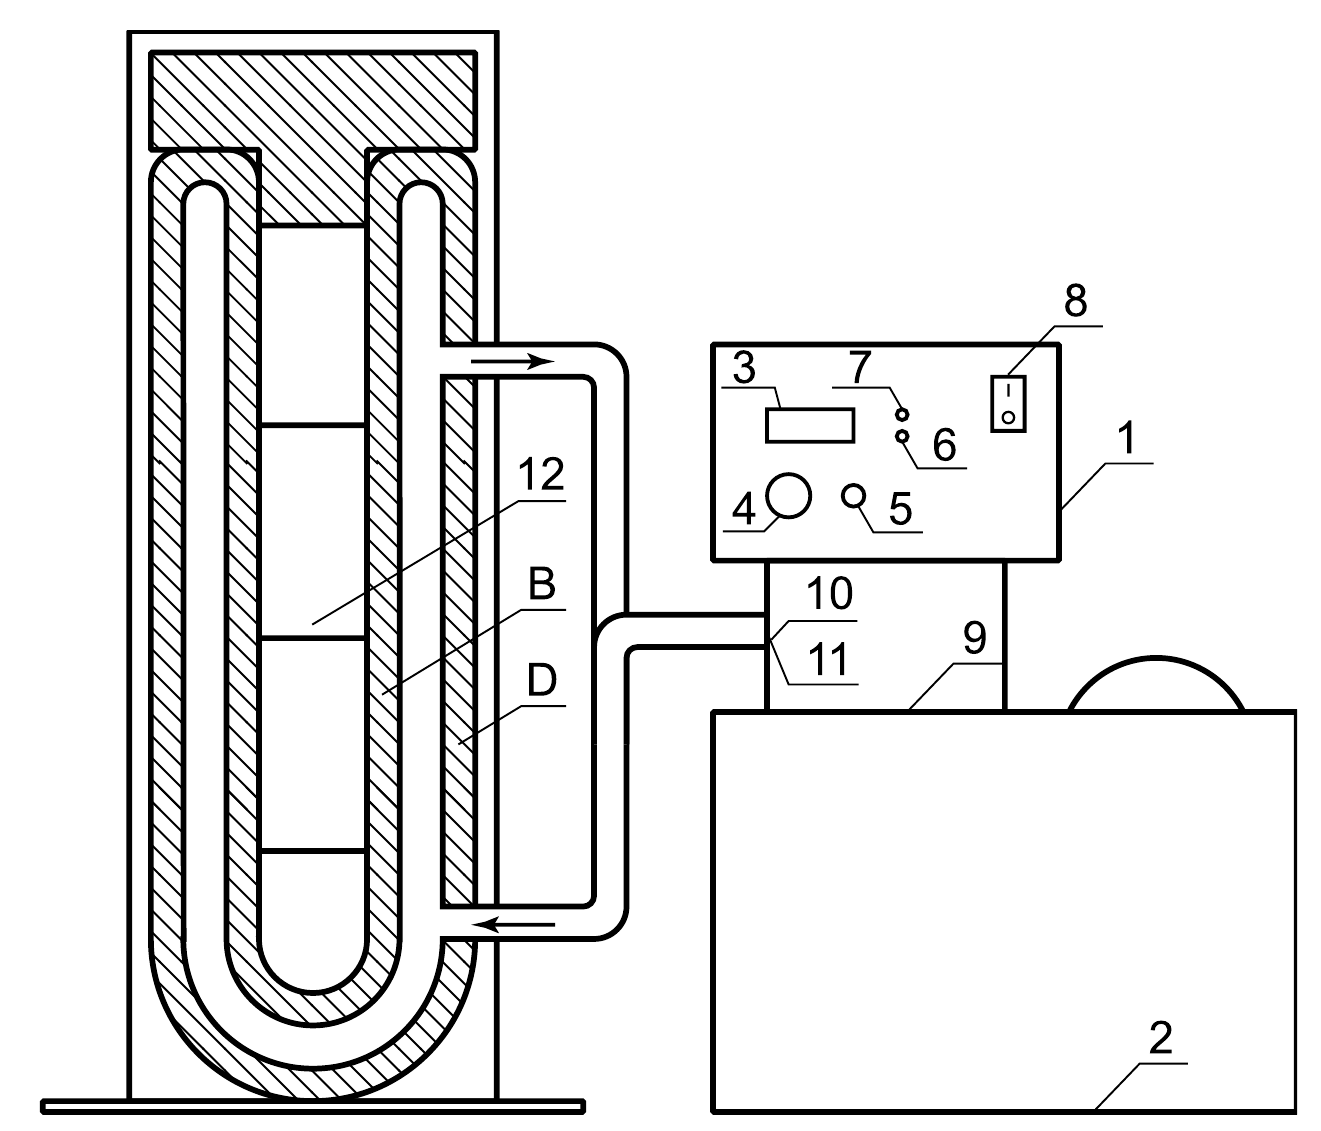
\includegraphics[width=0.6\linewidth]{setup}
		\caption{Схема установки:
			1 -  блок терморегулирования;
			2 - ванна;
			3 - индикаторное табло;
			4 - ручка установки температуры;
			5 - кнопка переключения режимов установки/контроля температуры;
			6 - индикатор уровня жидкости;
			7 - индикатор включения нагревателя;
			8 - сетевой выключатель прибора;
			9 - крышка;
			10 - входной и выходной патрубки насоса;
			11 - входной и выходной патрубки теплообменника (вода из водопровода);
			12 - исследуемая жидкость (глицерин).
			B - стеклянный сосуд;
			D - рубашка.
			}
		\label{fig:setup}
	\end{figure}
	
	
	Для измерений используется стеклянный цилиндрический сосуд В, наполненный исследуемой жидкостью 12, помещенный в рубашку, омываемую водой из термостата. На стенках сосуда нанесены две метки на некотором расстоянии друг от друга. Верхняя метка располагается ниже уровня жидкости, чтобы скорость шарика к моменту прохождения успевала установиться.
	
	
	\section*{Методика измерений}
	
	\hspace{4mm} Измеряя расстояние между метками с помощью линейки, а время падения с помощью секундомера, определяют скорость шарика $u$.
	
	
	Диаметры шариков измеряются горизонтальным компаратором
	или микроскопом несколько раз, и вычисляется среднее значение.
	
	
	Плотность шариков определяется из таблиц. Плотность исследуемой жидкости определяется
	по графику $\rho(T)$ на рис. 3.
	
	
	Опыты проводятся при нескольких температурах в интервале от
	комнатной до 50–60 $^o$C.

	
\section*{Результаты измерений}

\subsection*{Измерение диаметра шариков}

	\hspace{4mm} Результаты измерений диаметра шариков с помощью микроскопа представлены в табл. 1.

% Table generated by Excel2LaTeX from sheet 'Диаметры шариков'
\begin{table}[h!]
	\centering
	\captionbox{Диаметры шариков}{
	\begin{tabular}{|r|r|r|r|r|r|r|r|r|r|r|}
		\hline
		№ & 1 & 2        & 3        & 4        & 5        & 6        & 7        & 8        & 9        & 10        \\
		\hline
		$d_1, мм$ & 2,02 & 2,08     & 0,86     & 0,92     & 2,08     & 2,04     & 0,70     & 0,90     & 2,10     & 2,10     \\
		
		$d_2, мм$ & 2,10 & 2,10     & 0,82     & 0,96     & 2,06     & 2,10     & 0,72     & 0,92     & 2,06     & 2,04      \\
		
		$d_3, мм$ & 2,10 & 2,06     & 0,84     & 0,92     & 2,08     & 2,06     & 0,68     & 0,92     & 2,08     & 2,10      \\
		\hline
		$\bar{d}, мм$ & 2,07     & 2,08     & 0,84     & 0,93     & 2,07     & 2,07     & 0,70     & 0,91     & 2,08     & 2,08      \\
		\hline
		$\sigma_{сл}, мм$ & 0,038    & 0,016    & 0,016    & 0,019    & 0,009    & 0,025    & 0,016    & 0,009    & 0,016    & 0,028    \\
		\hline
		№        & 11       & 12       & 13       & 14       & 15       & 16       & 17       & 18       & 19       & 20 \\
		\hline
		$d_1, мм$ &  0,94     & 0,88     & 2,06     & 2,10     & 0,92     & 0,94     & 2,12     & 2,08     & 0,88     & 0,84 \\
		
		$d_2, мм$    & 0,94     & 0,90     & 2,12     & 2,08     & 0,94     & 0,92     & 2,08     & 2,10     & 0,90     & 0,82 \\
		
		$d_3, мм$     & 0,92     & 0,92     & 2,10     & 2,12     & 0,91     & 0,96     & 2,06     & 2,08     & 0,90     & 0,86 \\
		\hline
		$\bar{d}, мм$      & 0,93     & 0,90     & 2,09     & 2,10     & 0,92     & 0,94     & 2,09     & 2,09     & 0,89     & 0,84 \\
		\hline
		$\sigma_{сл}, мм$     & 0,009    & 0,016    & 0,025    & 0,016    & 0,012    & 0,016    & 0,025    & 0,009    & 0,009    & 0,016 \\
		\hline
	\end{tabular}}
	\label{tab:addlabe}%
\end{table}%

	Заметим, что для большинства шариков случайная погрешность измерения меньше систематической, поэтому трёх измерений было достаточно.

\subsection*{Измерение скорости падения шариков}

	\hspace{4mm} Расстояния между метками на колбе одинаковы и равны $(100 \pm 1) \ мм$. Поделив его на измеренное время, получаем среднюю скорость падения шарика (см. табл. 2).
	
	
	% Table generated by Excel2LaTeX from sheet 'Время падения'
	\begin{table}[htbp]
		\centering
		\captionbox{Скорости падения шариков}{
		\begin{tabular}{|r|r|r|r|r|r|r|r|r|r|r|}
			\hline
			№ & 1        & 2        & 3        & 4        & 5        & 6        & 7        & 8        & 9        & 10 \\
			\hline
			$v_1, мм/с$  & 3,12     & 3,10     & 2,47     & 3,08     & 6,96     & 7,03     & 3,87     & 6,47     & 13,76    & 13,99 \\
			
			$v_2, мм/с$ & 3,06     & 3,08     & 2,46     & 3,08     & 6,89     & 6,59     & 3,88     & 6,38     & 13,30    & 13,62 \\
			\hline
			$v, мм/с$ & 3,09     & 3,09     & 2,46     & 3,08     & 6,92     & 6,81     & 3,88     & 6,42     & 13,53    & 13,80 \\
			\hline
			$\sigma_{сл}, мм/с$ & 0,03     & 0,03     & 0,02     & 0,03     & 0,07     & 0,07     & 0,04     & 0,06     & 0,14     & 0,14 \\
			\hline
			№ & 11       & 12       & 13       & 14       & 15       & 16       & 17       & 18       & 19       & 20 \\
			\hline
			$v_1, мм/с$  & 14,53    & 15,60    & 23,75    & 26,11    & 26,04    & 25,25    & 40,32    & 45,05    & 33,11    & 38,02 \\
			
			$v_2, мм/с$  & 15,97    & 15,50    & 23,75    & 25,38    & 27,55    & 26,95    & 41,67    & 38,76    & 39,22    & 27,55 \\
			\hline
			$v, мм/с$  & 15,25    & 15,55    & 23,75    & 25,75    & 26,79    & 26,10    & 40,99    & 41,90    & 36,16    & 32,79 \\
			\hline
			$\sigma_{сл}, мм/с$  & 0,15     & 0,16     & 0,24     & 0,26     & 0,27     & 0,26     & 0,41     & 0,42     & 0,36     & 0,33 \\
			\hline
		\end{tabular}}
		\label{tab:addlabel}%
	\end{table}%
	
\subsection*{Определение вязкости}

	\hspace{4mm} Вязкость рассчитана по формуле (5) для каждого шарика (см. табл. 3). Разница вязкости между шариками разного радиуса (стеклянными и стальными) неразличима из-за погрешности, поэтому в уточнение по формуле (6) избыточно. Значения вязкости для каждой температуры усреднены по четырём шарикам. Так получена зависимость $\eta(t)$.

	\begin{table}[h!]
		\centering
		\captionbox{Зависимость вязкости глицерина от температуры}{
		\begin{tabular}{|c|r|r|r|r|c|}
			\hline
			\multirow{2}[4]{*}{t, $^oC$} & \multicolumn{2}{c|}{Стекло} & \multicolumn{2}{c|}{Сталь} & \multirow{2}[4]{*}{$\eta, Па \cdot с$} \\
			\cline{2-5}             & \multicolumn{1}{l|}{$\eta, Па \cdot с$} & \multicolumn{1}{l|}{$\sigma(\eta), Па \cdot с$} & \multicolumn{1}{l|}{$\eta, Па \cdot с$} & \multicolumn{1}{l|}{$\sigma(\eta), Па \cdot с$} &  \\
			\hline
			\multirow{2}[4]{*}{20} & 0,94     & 0,04     & 1,02     & 0,06     & \multirow{2}[4]{*}{0,98 $\pm$ 0,05} \\
			\cline{2-5}             & 0,95     & 0,03     & 1,01     & 0,06     &  \\
			\hline
			\multirow{2}[4]{*}{30} & 0,421    & 0,010    & 0,45     & 0,03     & \multirow{2}[4]{*}{0,44 $\pm$ 0,02} \\
			\cline{2-5}             & 0,426    & 0,014    & 0,46     & 0,02     &  \\
			\hline
			\multirow{2}[4]{*}{40} & 0,218    & 0,006    & 0,204    & 0,010    & \multirow{2}[4]{*}{0,205 $\pm$ 0,008} \\
			\cline{2-5}             & 0,213    & 0,007    & 0,186    & 0,011    &  \\
			\hline
			\multirow{2}[4]{*}{50} & 0,126    & 0,004    & 0,114    & 0,006    & \multirow{2}[4]{*}{0,119 $\pm$ 0,005} \\
			\cline{2-5}             & 0,117    & 0,003    & 0,121    & 0,007    &  \\
			\hline
			\multirow{2}[4]{*}{60} & 0,073    & 0,002    & 0,079    & 0,004    & \multirow{2}[4]{*}{0,075 $\pm$ 0,003} \\
			\cline{2-5}             & 0,071    & 0,002    & 0,077    & 0,005    &  \\
			\hline
		\end{tabular}}
		\label{tab:addla}%
	\end{table}%
	
	
\subsection*{Оценка погрешностей}
\hspace{4mm} Инструментальная погрешность измерения времени мала (0,01 с), а погрешность, связанную с реакцией наблюдателя, оценить сложно. Поэтому положим относительную погрешность скорости $\varepsilon_u \approx \varepsilon_s = 0,01$. 

Относительная погрешность измерения диаметра стеклянных шариков составила $\varepsilon_d(стекло) \approx 0,014$ и ожидаемо оказалась меньше, чем у стальных $\varepsilon_d(сталь) \approx 0,028$, так как их размер больше.

По формуле 5 оценим относительную погрешность измерения вязкости:

\begin{equation}
	\varepsilon(\eta) = \sqrt{4\varepsilon_r^2 + \varepsilon_u^2} \approx \sqrt{4\varepsilon_r^2 + 10^{-4}} \approx 0,04
\end{equation}	


\subsection*{Анализ применимости формулы Стокса}

\hspace{4mm} Для каждого эксперимента определены число Рейнольдса, время релаксации и её путь (см. табл. 4). Числа Рейнольдса малы, поэтому обтекание ламинарно. Путь релаксации меньше расстояния от поверхности жидкости до первой метки, поэтому скорость успевает установиться.

	% Table generated by Excel2LaTeX from sheet 'Лист1'
	\begin{table}[h!]
		\centering
		\captionbox{К анализу применимости формулы Стокса}{
		\begin{tabular}{|c|r|r|r|r|r|r|}
			\hline
			\multirow{2}[4]{*}{t, $^oC$} & \multicolumn{2}{c|}{Re} & \multicolumn{2}{c|}{$\tau, 0,1 c$} & \multicolumn{2}{c|}{$S, 0,1 мм$} \\
			\cline{2-7}             & \multicolumn{1}{l|}{Стекло} & \multicolumn{1}{l|}{Сталь} & \multicolumn{1}{l|}{Стекло} & \multicolumn{1}{l|}{Сталь} & \multicolumn{1}{l|}{Стекло} & \multicolumn{1}{l|}{Сталь} \\
			\hline
			\multirow{2}[4]{*}{20} & 0,004    & 0,0013   & 0,6      & 0,3      & 2,0      & 0,7 \\
			\cline{2-7}             & 0,004    & 0,0018   & 0,6      & 0,4      & 2,0      & 1,2 \\
			\hline
			\multirow{2}[4]{*}{30} & 0,021    & 0,0038   & 1,4      & 0,5      & 9,8      & 1,8 \\
			\cline{2-7}             & 0,021    & 0,0079   & 1,4      & 0,8      & 9,5      & 5,0 \\
			\hline
			\multirow{2}[4]{*}{40} & 0,081    & 0,0437   & 2,8      & 1,9      & 37,3     & 28,2 \\
			\cline{2-7}             & 0,084    & 0,0471   & 2,8      & 1,9      & 38,9     & 29,4 \\
			\hline
			\multirow{2}[4]{*}{50} & 0,246    & 0,1357   & 4,8      & 3,2      & 114,7    & 87,1 \\
			\cline{2-7}             & 0,288    & 0,1265   & 5,2      & 3,2      & 134,7    & 82,6 \\
			\hline
			\multirow{2}[4]{*}{60} & 0,730    & 0,2545   & 8,3      & 4,4      & 340,5    & 158,5 \\
			\cline{2-7}             & 0,763    & 0,2224   & 8,5      & 4,0      & 355,8    & 130,3 \\
			\hline
		\end{tabular}}
		\label{tab:addlab}%
	\end{table}%
	
	
\subsection*{Построение графика $\ln(\eta) = f(1/T)$}

\begin{figure}[h!]
	\centering
	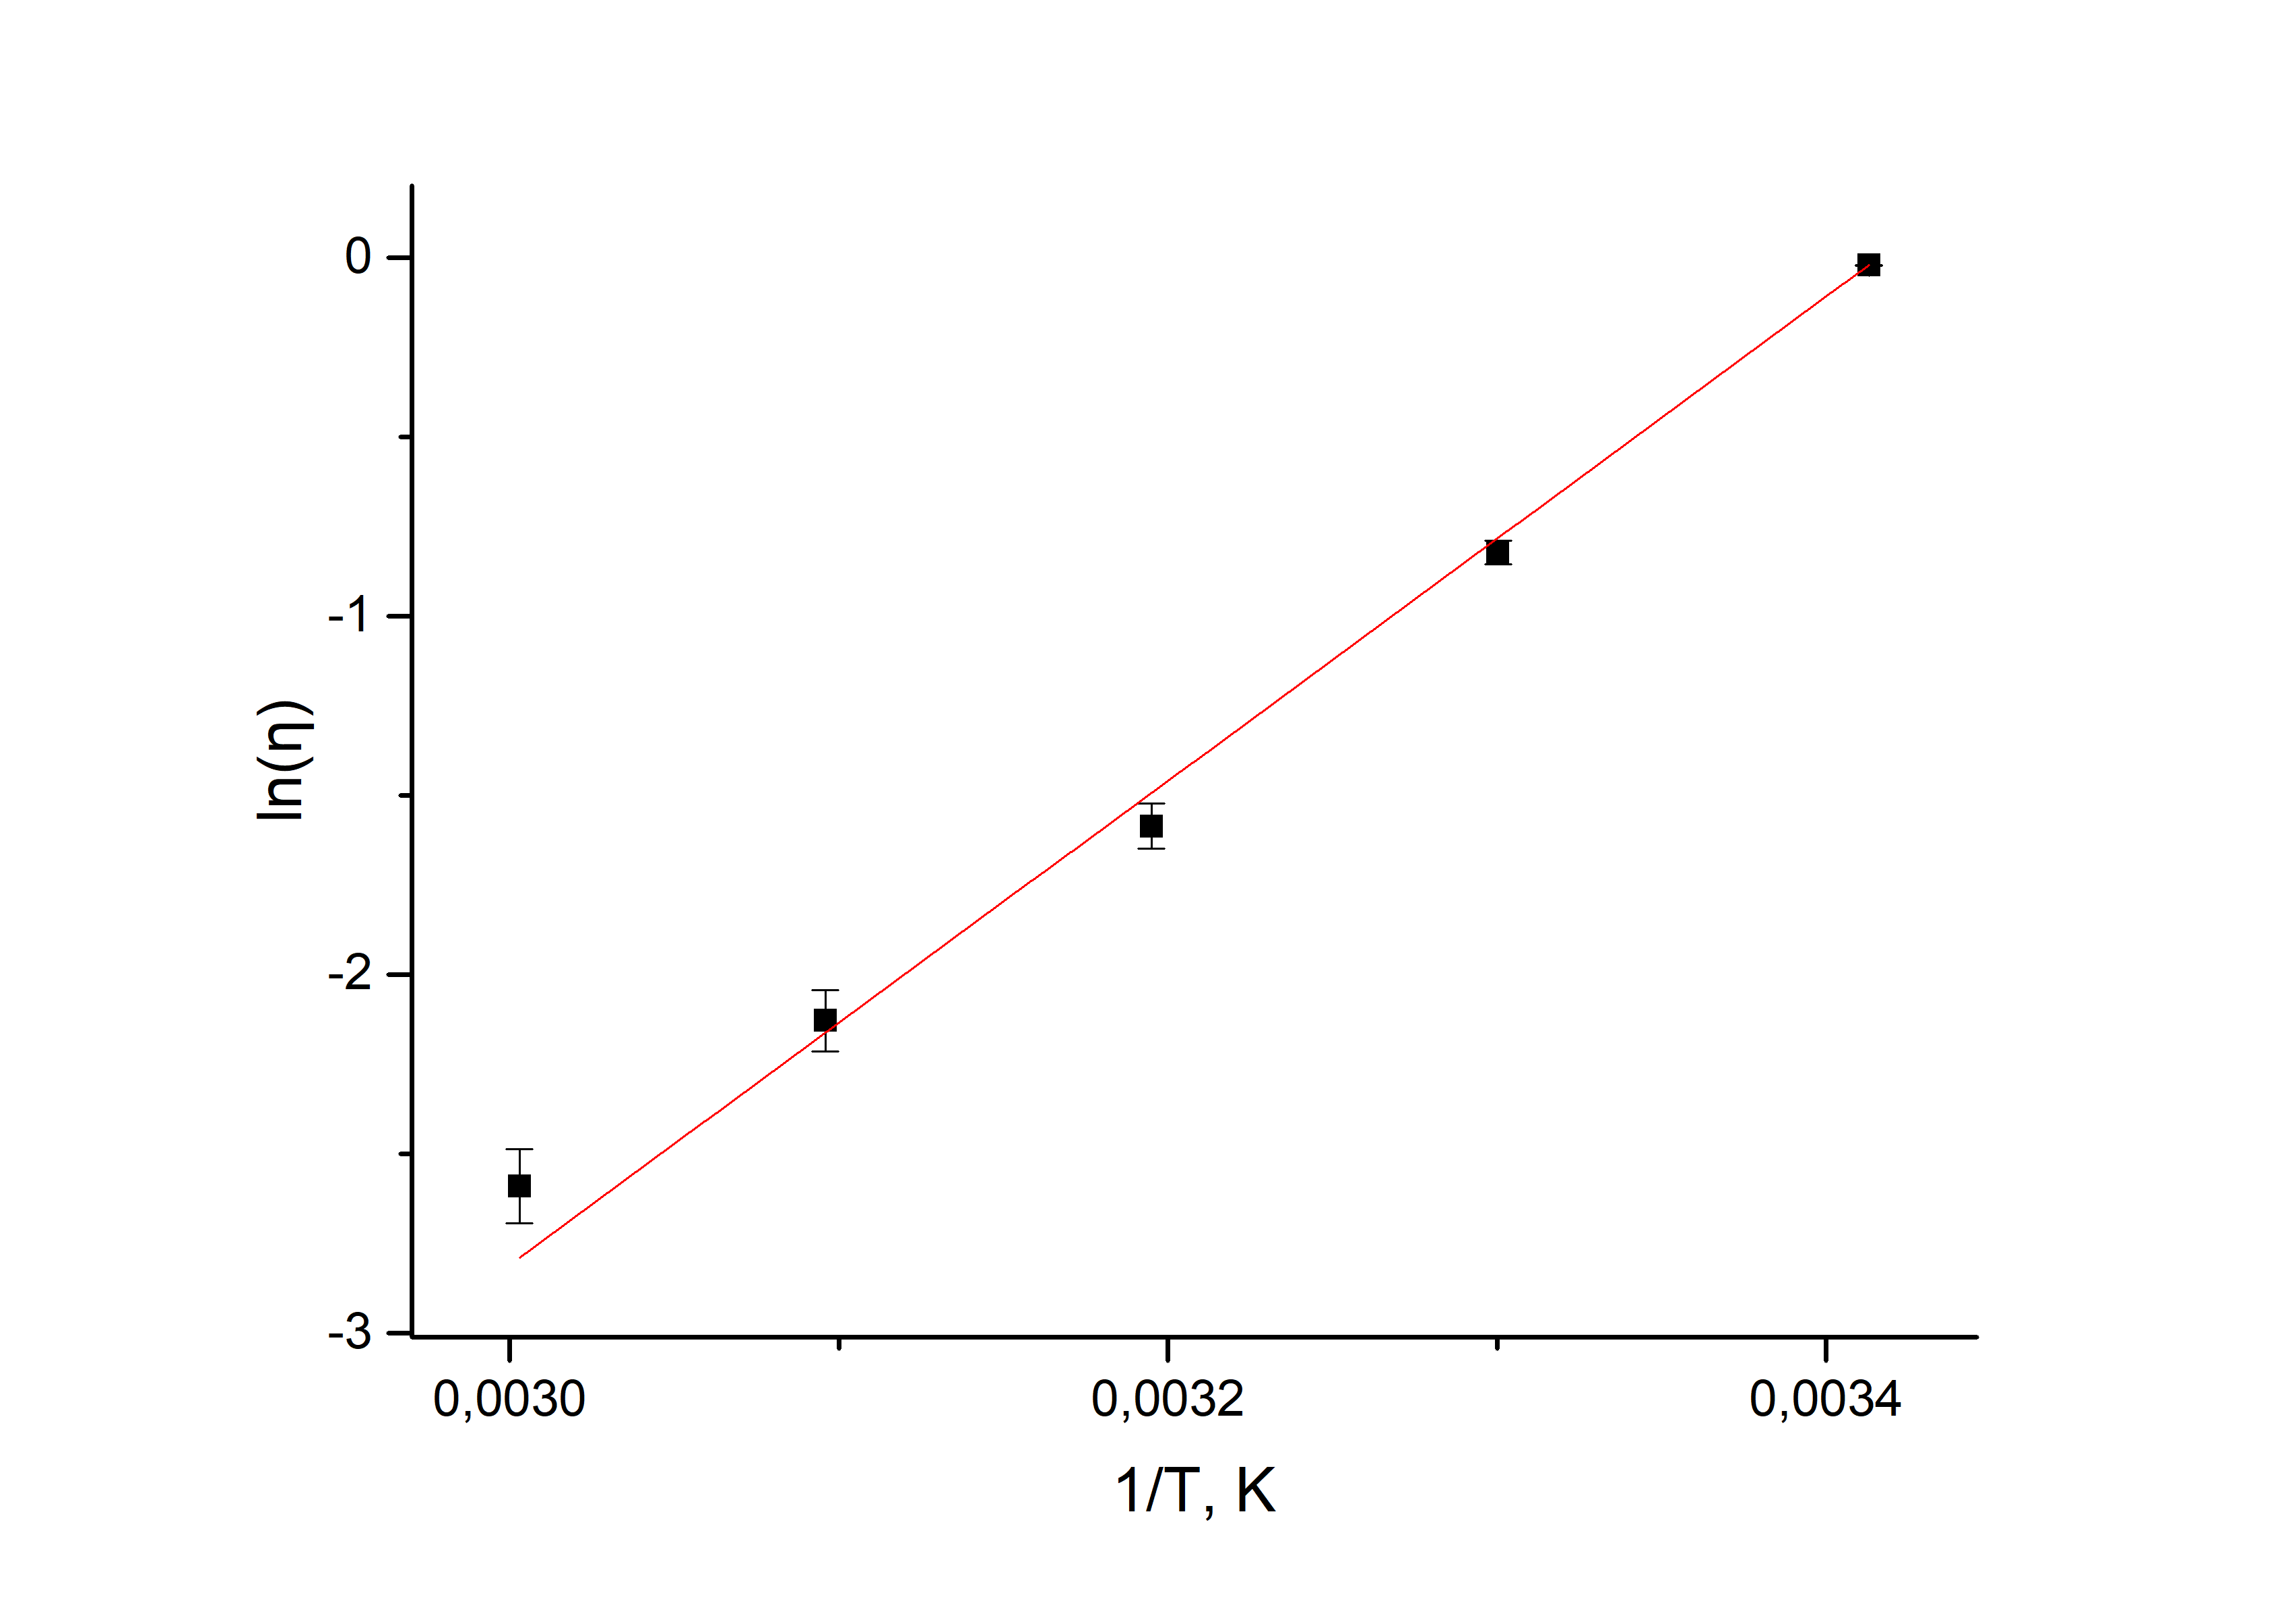
\includegraphics[width=0.85\linewidth]{plot}
	\caption{График $\ln(\eta) = f(1/T)$}
	\label{fig:plot}
\end{figure}


	\hspace{4mm} Логарифмируя уравнение (1) имеем
	
	\begin{equation}
		\ln(\eta) = \ln(A) + \frac{W}{kT}.
	\end{equation}
	
	Таким образом, построив график в координатах $\ln(\eta)$ и $1/T$ (см. рис. 2) и проведя наилучшую прямую $ln(\eta) = a(1/T) + b$, мы определим энергию активации молекулы $W = ka$.
	
	
	\begin{equation*}
		a = (6,6 \pm 0,2) \ К, \ \ \ k \approx 1,38 \cdot 10^{-23} \ Дж/К
	\end{equation*}
	
	\begin{equation*}
		W = (9,1 \pm 0,3) \cdot 10^{-20} \ Дж
	\end{equation*}
	
	В пересчёте на один моль (умножением на постоянную Авогадро $N_A = 6,022 \cdot 10^{23} 1/моль$)
	
	\begin{equation*}
		\boxed{W = (54,6 \pm 1,8)  \ кДж/моль}
	\end{equation*}

	
\section*{Заключение}

	\hspace{4mm} Найденные значения вязкости глицерина при разных температурах хорошо согласуются со справочными данными. Немногочисленные источники дают разные значения энергии активации глицерина: 46 - 77 кДж/моль. Полученное значение попадает в этот диапазон.
	
	Относительная погрешность результата составила меньше 4\%. Основной вклад внесла погрешность измерения радиуса шаров. Кроме того, вызывает сомнения методика измерения времени падения шариков: невозможно оценить погрешность, связанную со скоростью реакции наблюдателя, между тем она явно не пренебрежимо мала, особенно в последних опытах. Устранить этот источник погрешности можно, например, с помощью датчиков на оптопаре или увеличением высоты колбы.
	
	Цели работы достигнуты: измерены скорости падения шариков при разной температуре глицерина, вычислена вязкости жидкости и найдена энергия активации.
	
		
\end{document}